\documentclass{standalone}

%----------------------------------------------------------------------------------------------%
%                                 Packages and basic declarations
%----------------------------------------------------------------------------------------------%

\usepackage[utf8]{inputenc}
\usepackage{pgfplots}
\usepackage{tikz}


%----------------------------------------------------------------------------------------------%
%----------------------------------------------------------------------------------------------%
%                                            DOCUMENT STARTS
%----------------------------------------------------------------------------------------------%
%----------------------------------------------------------------------------------------------%

\begin{document}


%Tikz picture starts%

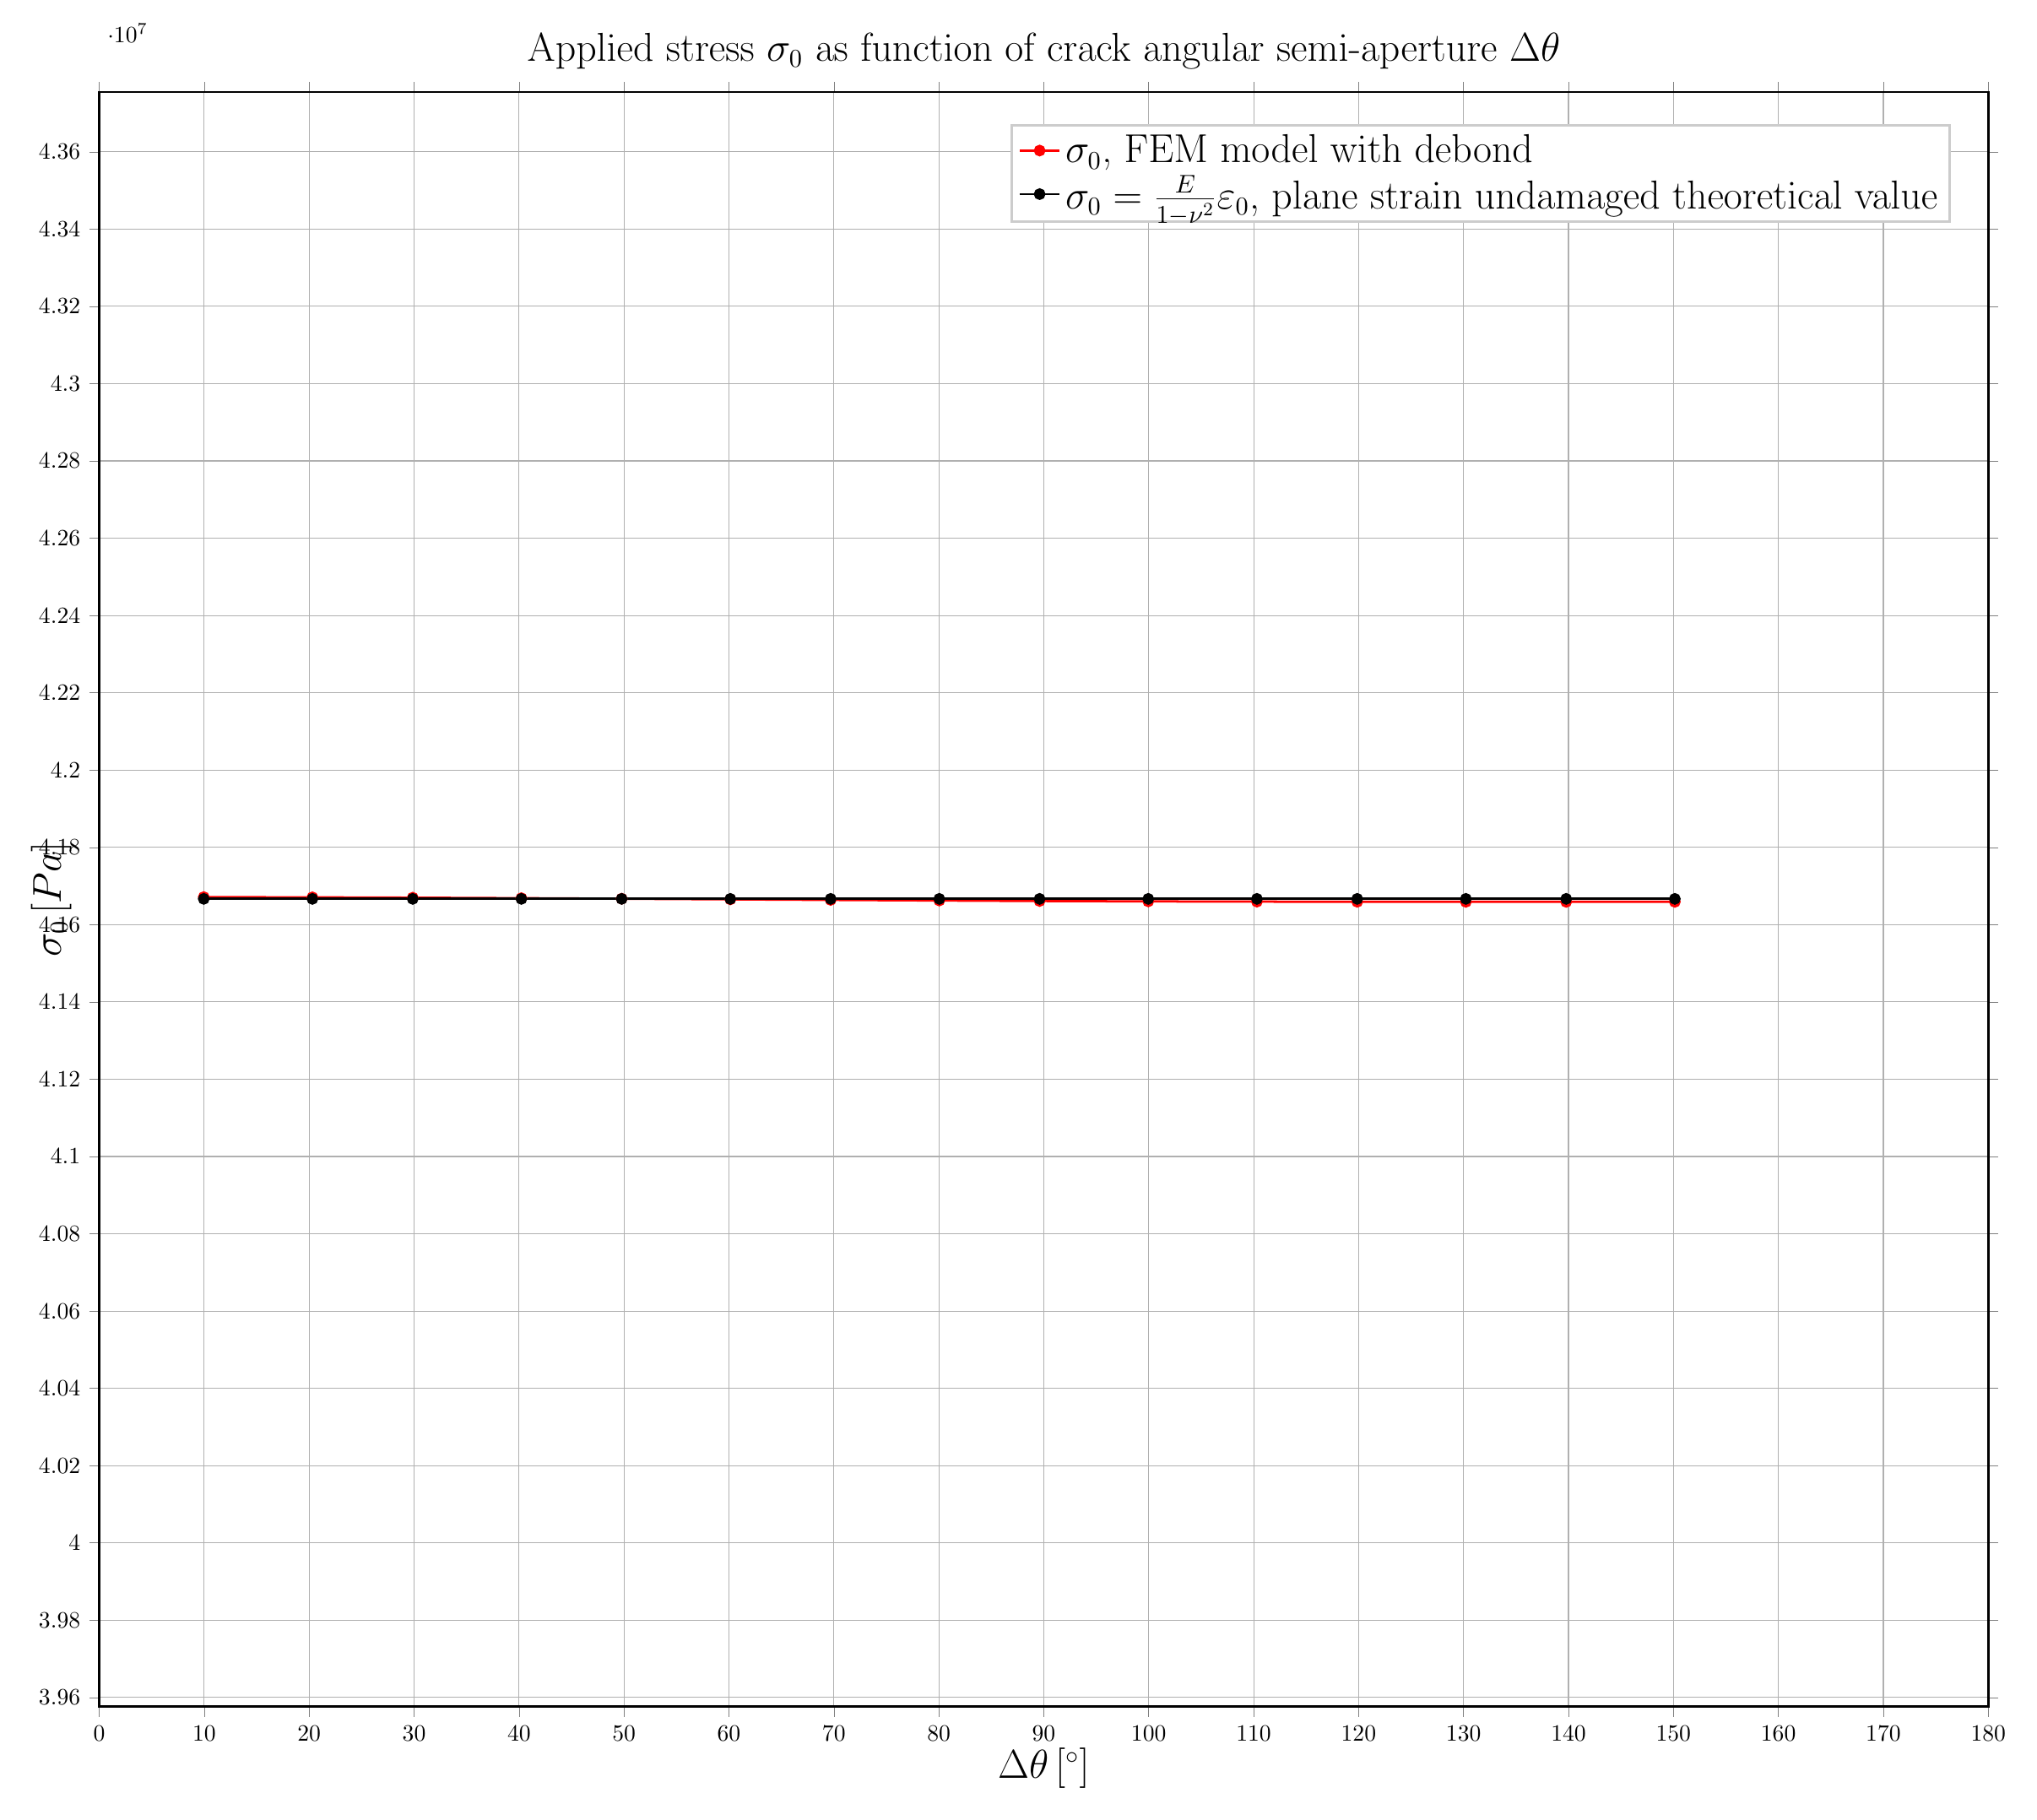
\begin{tikzpicture}

%Tikz axis starts%

\begin{axis}[width=30cm,
title={Applied stress $\sigma_{0}$ as function of crack angular semi-aperture  $\Delta\theta$},
title style={font=\fontsize{16}{8}\selectfont},
xlabel style={at={(axis description cs:0.5,-0.02)},anchor=north,font=\fontsize{16}{8}\selectfont},
ylabel style={at={(axis description cs:-0.01,.5)},anchor=south,font=\fontsize{16}{8}\selectfont},
xlabel={$\Delta\theta\left[^{\circ}\right]$},ylabel={$\sigma_{0}\left[Pa\right]$},
xmin=0.0,
xmax=180.0,
ymin=39576042.8906,
ymax=43754832.8701,
tick align=outside,
tick label style={font=\normalsize},
xtick={0.0,10.0,20.0,30.0,40.0,50.0,60.0,70.0,80.0,90.0,100.0,110.0,120.0,130.0,140.0,150.0,160.0,170.0,180.0},
xmajorgrids,
x grid style={lightgray!92.026143790849673!black},
ymajorgrids,
y grid style={lightgray!92.026143790849673!black},
line width=0.35mm,
legend style={draw=white!80.0!black,font=\fontsize{16}{12}\selectfont},
legend entries={{$\sigma_{0}$, FEM model with debond},{$\sigma_{0}=\frac{E}{1-\nu^{2}}\varepsilon_{0}$, plane strain undamaged theoretical value}},
legend cell align={left}
]

\addplot[red,smooth,mark=*]
table{
9.95590315404 41671269.4001
20.3094667517 41670638.4358
29.8671878064 41669719.2778
40.2210818145 41668431.3657
49.7789172749 41667052.6203
60.1328146981 41665452.5723
69.6905306301 41663966.5135
80.044093374 41662446.1057
89.6017683249 41661187.1468
99.9559048047 41660217.9042
110.309467549 41659548.9602
119.867183481 41659205.4367
130.221080904 41659046.3069
139.778919779 41659007.7752
150.132817203 41659004.0107
};

\addplot[black,smooth,mark=*]
table{
9.95590315404 41666666.6667
20.3094667517 41666666.6667
29.8671878064 41666666.6667
40.2210818145 41666666.6667
49.7789172749 41666666.6667
60.1328146981 41666666.6667
69.6905306301 41666666.6667
80.044093374 41666666.6667
89.6017683249 41666666.6667
99.9559048047 41666666.6667
110.309467549 41666666.6667
119.867183481 41666666.6667
130.221080904 41666666.6667
139.778919779 41666666.6667
150.132817203 41666666.6667
};

\end{axis}
%Tikz axis ends%


\end{tikzpicture}
%Tikz picture ends%


\end{document}

%----------------------------------------------------------------------------------------------%
%----------------------------------------------------------------------------------------------%
%                                            DOCUMENT ENDS
%----------------------------------------------------------------------------------------------%
%----------------------------------------------------------------------------------------------%

